%für Sprache, A4 Blatt, float, Grafiken, UTF Codierung, PDF, Color, Seitenabstand, Listings
\documentclass[a4papr,12pt]{article}
\usepackage[utf8]{inputenc}
\usepackage[ngerman]{babel}
\usepackage{graphicx}
\usepackage{float}
\usepackage{textcomp}
\usepackage{pdfpages}
\usepackage{tikz}
\usepackage{hyperref}
\usepackage{geometry}
\usepackage{listings}
\usepackage{color}
\usepackage{grffile}

%Mathematics
\usepackage{amstext}
\usepackage{amssymb}
\usepackage{amsmath}
\usepackage{amsfonts}
\usepackage{mathrsfs}
\usepackage{mathtools}

%include this before fancy or page style gets messed up bc of geometry
%Seitenabstand A4 Blatt
\geometry{a4paper}
\geometry{top=25mm,bottom=25mm,left=23mm,right=20mm}

% macro to select a scaled-down version of Bera Mono (for instance)
\makeatletter
\newcommand\BeraMonottfamily{%
  \def\fvm@Scale{0.85}% scales the font down
  \fontfamily{fvm}\selectfont% selects the Bera Mono font
}
\makeatother

%Hyperref zum anklicken von Überschriften in Texmaker + Farben einstellen
\hypersetup{
	colorlinks,
	citecolor=black,
	filecolor=black,
	linkcolor=blue,
	urlcolor=black
}

\definecolor{mygreen}{rgb}{0,0.6,0}
\definecolor{mygray}{rgb}{0.5,0.5,0.5}
\definecolor{mymauve}{rgb}{0.58,0,0.82}

%Zum Pascal Code einfügen mit lstinputlisting[language=Pascal] {../blabla.pas}
\lstset{ %
  backgroundcolor=\color{white},   % choose the background color; you must add \usepackage{color} or 								  \usepackage{xcolor}
  basicstyle=\BeraMonottfamily,        % the size of the fonts that are used for the code
  breakatwhitespace=false,         % sets if automatic breaks should only happen at whitespace
  breaklines=true,                 % sets automatic line breaking
  captionpos=b,                    % sets the caption-position to bottom
  commentstyle=\color{mygreen},    % comment style
  deletekeywords={...},            % if you want to delete keywords from the given language
  escapeinside={\%*}{*)},          % if you want to add LaTeX within your code
  extendedchars=true,              % lets you use non-ASCII characters; for 8-bits encodings only, 												does not work with UTF-8
  frame=single,	               % adds a frame around the code
  keepspaces=true,                 % keeps spaces in text, useful for keeping indentation of code 									  (possibly needs columns=flexible)
  keywordstyle=\color{blue},       % keyword style
  language=Octave,                 % the language of the code
  otherkeywords={...},           % if you want to add more keywords to the set
  numbers=left,                    % where to put the line-numbers; possible values are (none, left, 								  right)
  numbersep=5pt,                   % how far the line-numbers are from the code
  numberstyle=\tiny\color{black}, % the style that is used for the line-numbers
  rulecolor=\color{black},         % if not set, the frame-color may be changed on line-breaks within 								  not-black text (e.g. comments (green here))
  showspaces=false,                % show spaces everywhere adding particular underscores; it 														overrides 'showstringspaces'
  showstringspaces=false,          % underline spaces within strings only
  showtabs=false,                  % show tabs within strings adding particular underscores
  stepnumber=2,                    % the step between two line-numbers. If it's 1, each line will be 								  numbered
  stringstyle=\color{mymauve},     % string literal style
  title=\getlstname,
  tabsize=2,	                    % sets default tabsize to 2 spaces
  inputencoding=latin1,
  columns=fullflexible
}

\lstset{literate=%
	{Ö}{{\"O}}1
	{Ä}{{\"A}}1
	{Ü}{{\"U}}1
	{ß}{{\ss}}1
	{ü}{{\"u}}1
	{ä}{{\"a}}1
	{ö}{{\"o}}1
	{~}{{\textasciitilde}}1
}

%Filenamen und Pfad trennen
\makeatletter
\DeclareRobustCommand{\getlstname}{%
\begingroup
  % \lstname seems to change hyphens into \textendash
  \def\textendash{-}%
  \filename@parse{\lstname}%
  \texttt{\filename@base.\filename@ext}%
\endgroup
}


%Für Kopfzeile den Style
\usepackage{fancyhdr}
\pagestyle{fancy}
\lhead{ADE - Übung 8}
\rhead{Andreas Roither, \today{}}
\newcommand{\Cross}{\mathbin{\tikz [x=1.4ex,y=1.4ex,line width=.2ex] \draw (0,0) -- (1,1) (0,1) -- (1,0);}}%

\begin{document}

%ANGABE     
\thispagestyle{plain}
\includepdf[pages={1},pagecommand={     
\begin{tikzpicture}[remember picture, overlay]\node at (15.8, -1.35) {10 h};\end{tikzpicture}
\begin{tikzpicture}[remember picture, overlay]\node at (7.6, -1.35) {Andreas Roither};\end{tikzpicture}
\begin{Huge}
\begin{tikzpicture}[remember picture, overlay]\node at (-1.3, -1.9) {X};\end{tikzpicture}
\end{Huge}
}]{Angabe/Uebung08.pdf}
\includepdf[pages=2-,pagecommand={}]{Angabe/Uebung08.pdf}

\section*{Übung 8}
\subsection*{Aufgabe 1}
\subsubsection*{Lösungsidee}
Es sollen beliebig große ganze Zahlen addiert und multipliziert werden. Dazu wird eine Liste verwendet in der Nodes sind, die einen Integer mit maximal drei Stellen beinhalten. Diese Integer der Nodes zusammen gezählt ergeben die Zahl, wobei die erste Node die untersten drei Stellen der Zahl und die letzte Node die größten drei Stellen der Zahl beinhaltet. Für das Addieren und multiplizieren werden eigene Funktionen erstellt denen BigInPtr übergeben werden. Damit auch negative Zahlen addiert werden können, wird eine Funktion  HigherBigInt verwendet die zurückgibt welche Zahl größer ist bzw. ob beide gleich sind. Je nachdem was dies Funktion zurückliefert wird unterschiedlich gerechnet. Für das allgemeine Addieren werden die Integer der Nodes zusammen gezählt und mit einem overflow Integer zusammengezählt. Ist diese Summe größer als 999 muss bei der nächsten Node + 1 dazu gezählt werden, daher wird overflow auf 1 gesetzt. Bei negativen Zahlen wird überprüft ob die Summe unter 0 ist. Falls dies der Fall ist wird overflow auf -1 gesetzt und bei der nächsten Node subtrahiert.
\newline

\lstinputlisting[language=Pascal] {../BigInts.pas}
\begin{figure}[H]
	\centering
	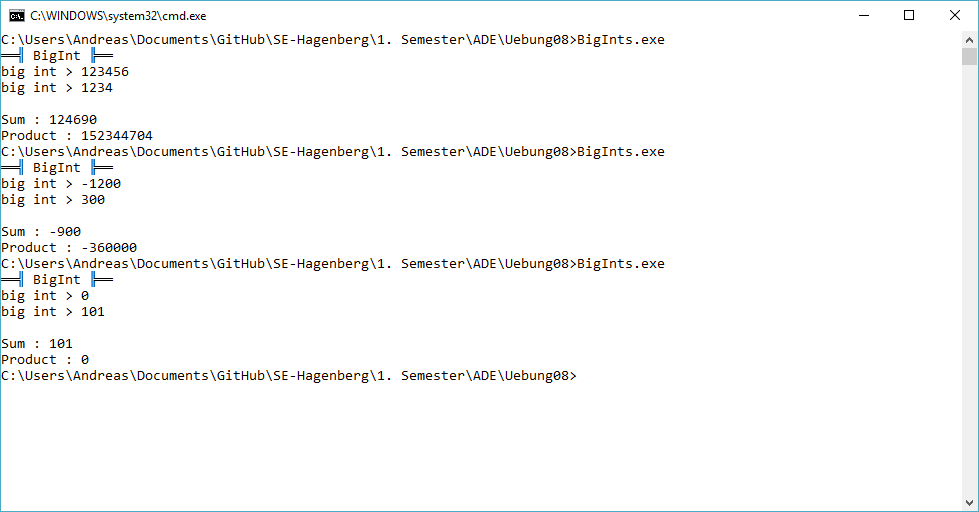
\includegraphics[scale=0.65]{./pictures/BigInts.png}
	\caption{Testfälle BigInts}
	\label{fig: BigInts}
\end{figure}

\section*{Testfälle}
Die Testfälle zeigen die Addition / Multiplikation mit positiven und negativen Zahlen. Das Addieren funktioniert solange genug Speicher für die Liste vorhanden ist. Beim Multiplizieren wird ein Laufzeitfehler verursacht wenn der Maximale Wertebereich von Int64 unter/überschritten wird. Alternativ kann hier mit einem String gearbeitet werden, jedoch ist dieser auch \grqq beschränkt\grqq{} auf 255 Zeichen,  \grqq unendlich lange\grqq{} Zahlen können damit aber nicht verwirklicht werden.
\newpage

\subsection*{Aufgabe 2}
\subsubsection*{Lösungsidee}
Bei dieser Aufgabe wird eine Wish List erstellt die Wünsche von einem Text Dokument einliest. Aufgrund dieser Liste wird eine Order Liste erstellt. In dieser sind alle Dinge die sich die Kinder wünschen Mengenmäßig enthalten. Danach wird eine Delivery Liste erstellt, in der alle Wünsche für das jeweilige Kind enthalten ist. Es werden für die Ausgabe, Node-erstellung und anfügen an eine Liste Funktionen bzw. Prozeduren erstellt.
\newline

\lstinputlisting[language=Pascal] {../WLA.pas}
\begin{figure}[H]
	\centering
	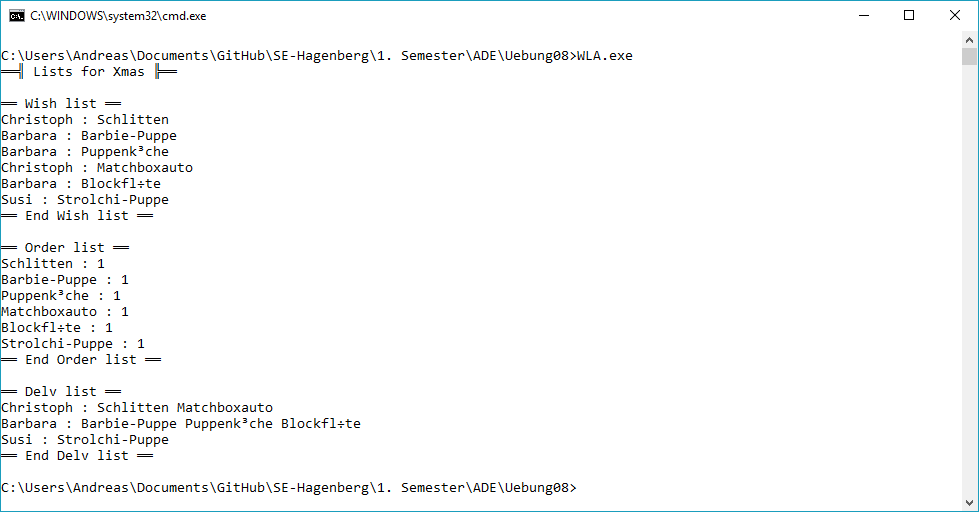
\includegraphics[scale=0.65]{./pictures/XMAS.png}
	\caption{Testfälle WLA}
	\label{fig: WLA}
\end{figure}

\section*{Testfall}
Hier wird gezeigt, dass die WishList die Wünsche der Kinder aus dem Textdokument enthält. Die OrderList wird aufgrund dieser Liste erzeugt. Die DeliveryList enthält Kinder mit ihren Wünschen basierend auf der WishList.
\newpage





\end{document}





